
\documentclass[11pt,a4paper]{article}
\usepackage[margin=1.1in]{geometry}
\usepackage{amsmath, amssymb, amsthm}
\usepackage{graphicx}
\usepackage{booktabs}
\usepackage{siunitx}
\usepackage{hyperref}
\usepackage{microtype}
\usepackage{physics}
\usepackage{csquotes}
\usepackage{caption}
\usepackage{listings}
\usepackage{xcolor}

\hypersetup{colorlinks=true,linkcolor=blue,citecolor=blue,urlcolor=blue}
\title{Finding a Whisper in a Storm: An Intuitive Walkthrough of LIGO-Style Matched Filtering}
\author{}
\date{\today}

\begin{document}
\maketitle

\begin{abstract}
Gravitational waves are faint ripples in spacetime, so faint that even the most sensitive instruments see mostly noise. This document tells the story of how data analysis---especially matched filtering---turns noisy strain measurements into confident detections. We build a minimal, reproducible ``toy detector'': a synthetic chirp signal hidden inside random noise. We then recover it using the very idea at the heart of LIGO's searches. The goal is not to recite names and dates, but to \emph{understand why} the method works, what ``Gaussian'' really means for noise, and how the whole pipeline hangs together from intuition to result.
\end{abstract}

\section{The Problem: Hearing a Pattern You Expect}
Imagine a melody played once in a noisy room. If you know the melody in advance, you can ``listen for it.'' Matched filtering formalizes this idea. We assume we know the general shape of the signal we seek (a template); we slide that template across the data and measure how well they line up at every time. Where alignment is best, the template ``rings,'' producing a peak in a detection statistic.

\section{Generative Model and Hypotheses}
We model the observed strain $d(t)$ as either noise alone or noise plus a signal:
\begin{align}
\mathcal{H}_0:~ d(t) &= n(t), \label{eq:h0}\\
\mathcal{H}_1:~ d(t) &= h(t) + n(t), \label{eq:h1}
\end{align}
where $n(t)$ is a (roughly) stationary random process and $h(t)$ is a deterministic pattern predicted by physics (our template).

If the noise is (approximately) Gaussian, then the likelihood ratio between $\mathcal{H}_1$ and $\mathcal{H}_0$ can be expressed in terms of a noise-weighted inner product. In continuous frequency language, define
\begin{equation}
(a|b) \equiv 4\,\Re \int_{0}^{\infty} \frac{\tilde a(f)\,\tilde b^{*}(f)}{S_n(f)}\,\mathrm{d}f, \label{eq:inner}
\end{equation}
where tildes denote Fourier transforms and $S_n(f)$ is the (one-sided) noise power spectral density (PSD).

\section{Matched Filtering and SNR}
For a template $h$ (allowing a relative time shift $\tau$), the matched-filter signal-to-noise ratio (SNR) time series is
\begin{equation}
\rho(\tau) \equiv \frac{(d | h_\tau)}{\sqrt{(h|h)}}, \qquad
h_\tau(t) \equiv h(t-\tau). \label{eq:snr}
\end{equation}
Peaks of $\rho(\tau)$ indicate times where $d$ contains $h$ most strongly, with the weighting in \eqref{eq:inner} downweighting frequencies where the detector is noisier.

\section{What ``Gaussian Noise'' Really Means}
``Gaussian'' is about a \emph{shape} that randomness tends to take. A process is Gaussian when any linear combination of samples is normally distributed; empirically, histograms of noise-only samples form a bell-shaped curve. In practice, this means averages and correlations are predictable: the central limit effect makes extreme fluctuations rare and typical fluctuations well-characterized by a mean and standard deviation.

\section{Whitening and Spectrograms}
To make features visually apparent and to approximate the weighting in \eqref{eq:inner}, we \emph{whiten} the data: we estimate $S_n(f)$ and flatten the spectrum via
\begin{equation}
\tilde x_{\mathrm{w}}(f) \equiv \frac{\tilde x(f)}{\sqrt{S_n(f)}}, \qquad
x_{\mathrm{w}}(t) = \mathcal{F}^{-1}\!\big[\tilde x_{\mathrm{w}}(f)\big], \label{eq:whiten}
\end{equation}
where $\mathcal{F}^{-1}$ is the inverse Fourier transform. We then compute a short-time Fourier transform (STFT),
\begin{equation}
Z(t_k,f_m) \equiv \sum_{t} x_{\mathrm{w}}(t)\,w(t-t_k)\,e^{-i2\pi f_m t}, \label{eq:stft}
\end{equation}
with a long window and high overlap to reduce variance. We visualize $10\log_{10}|Z|^2$ after subtracting, for each frequency $f_m$, the median over $t_k$ (this removes stationary backgrounds):
\begin{equation}
S_{\mathrm{dB}}^{\mathrm{ms}}(t_k,f_m) \equiv 10\log_{10}\!\big(|Z(t_k,f_m)|^2\big)
~ - ~ \mathrm{median}_{t_k}\!\left[\,10\log_{10}\!\big(|Z(t_k,f_m)|^2\big)\,\right]. \label{eq:medsub}
\end{equation}
Finally, we apply a contrast stretch by clipping the color scale to the $95$th--$99.5$th percentiles of $S_{\mathrm{dB}}^{\mathrm{ms}}$ before plotting. This emphasizes the faint, time-varying structure of the chirp.

\section{Doing It: From Data to Detection}
We compute the (toy) matched filter output and identify the peak as the estimated arrival time, while the whitened, median-subtracted spectrogram highlights the rising-frequency pattern of the hidden chirp.

\begin{figure}[h!]
\centering
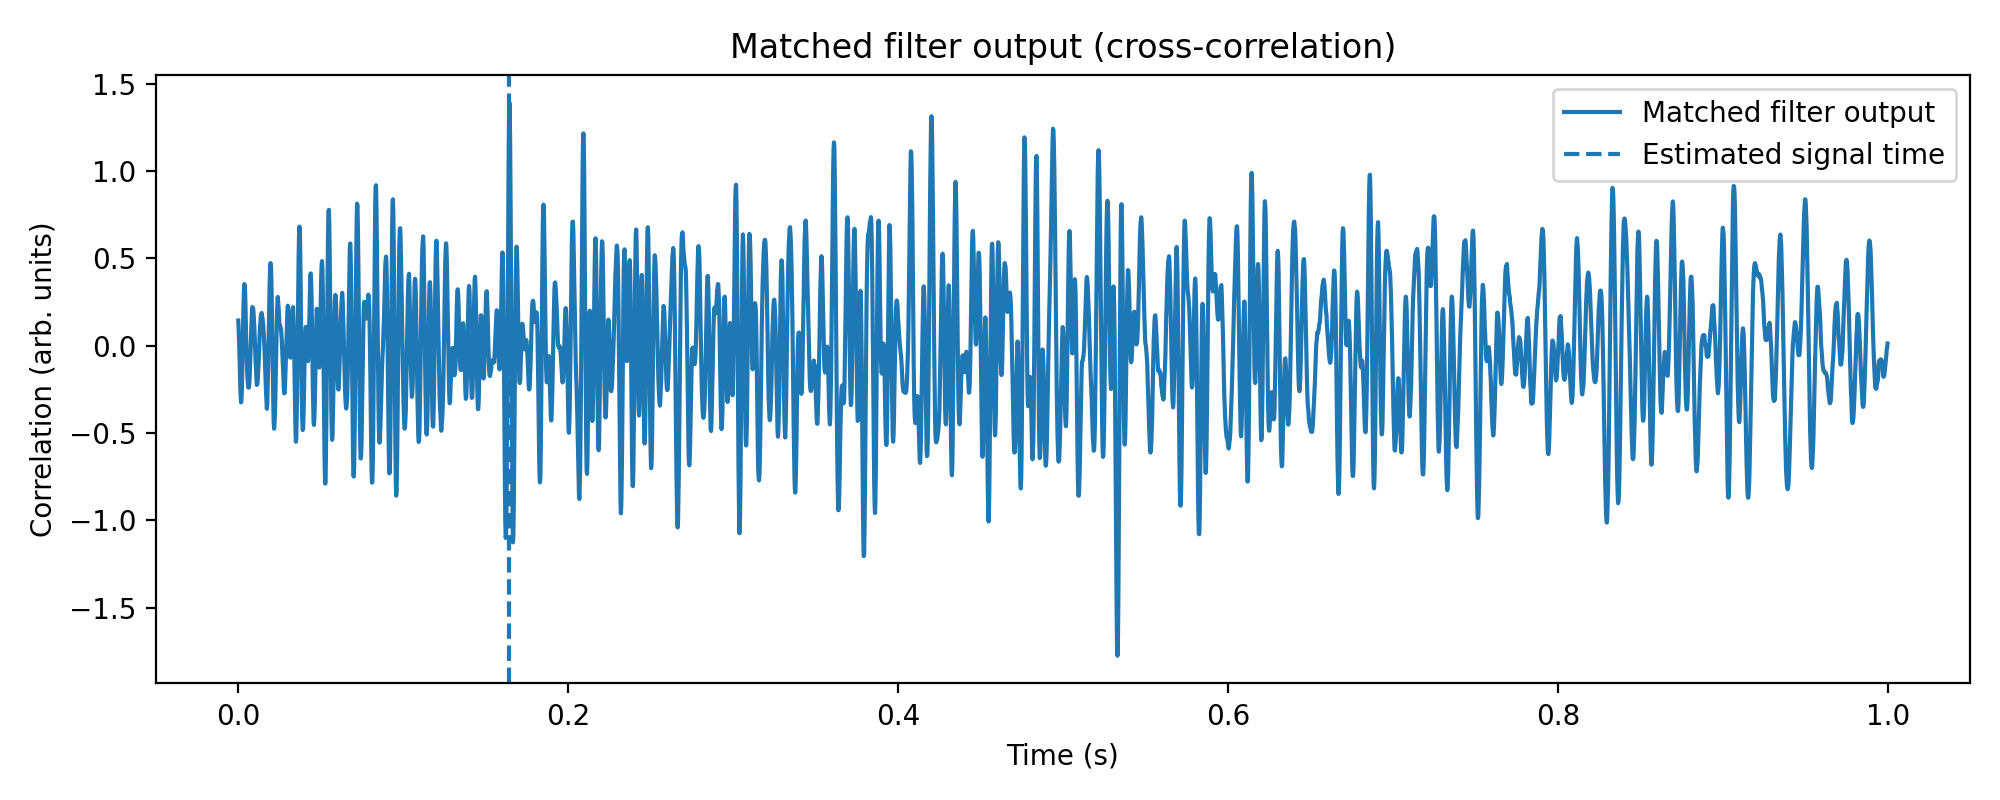
\includegraphics[width=0.95\linewidth]{fig2_correlation.png}
\caption{Matched-filter output (correlation) vs.\ time. The dashed line marks the peak, which estimates the signal arrival time.}
\label{fig:corr}
\end{figure}

\begin{figure}[h!]
\centering
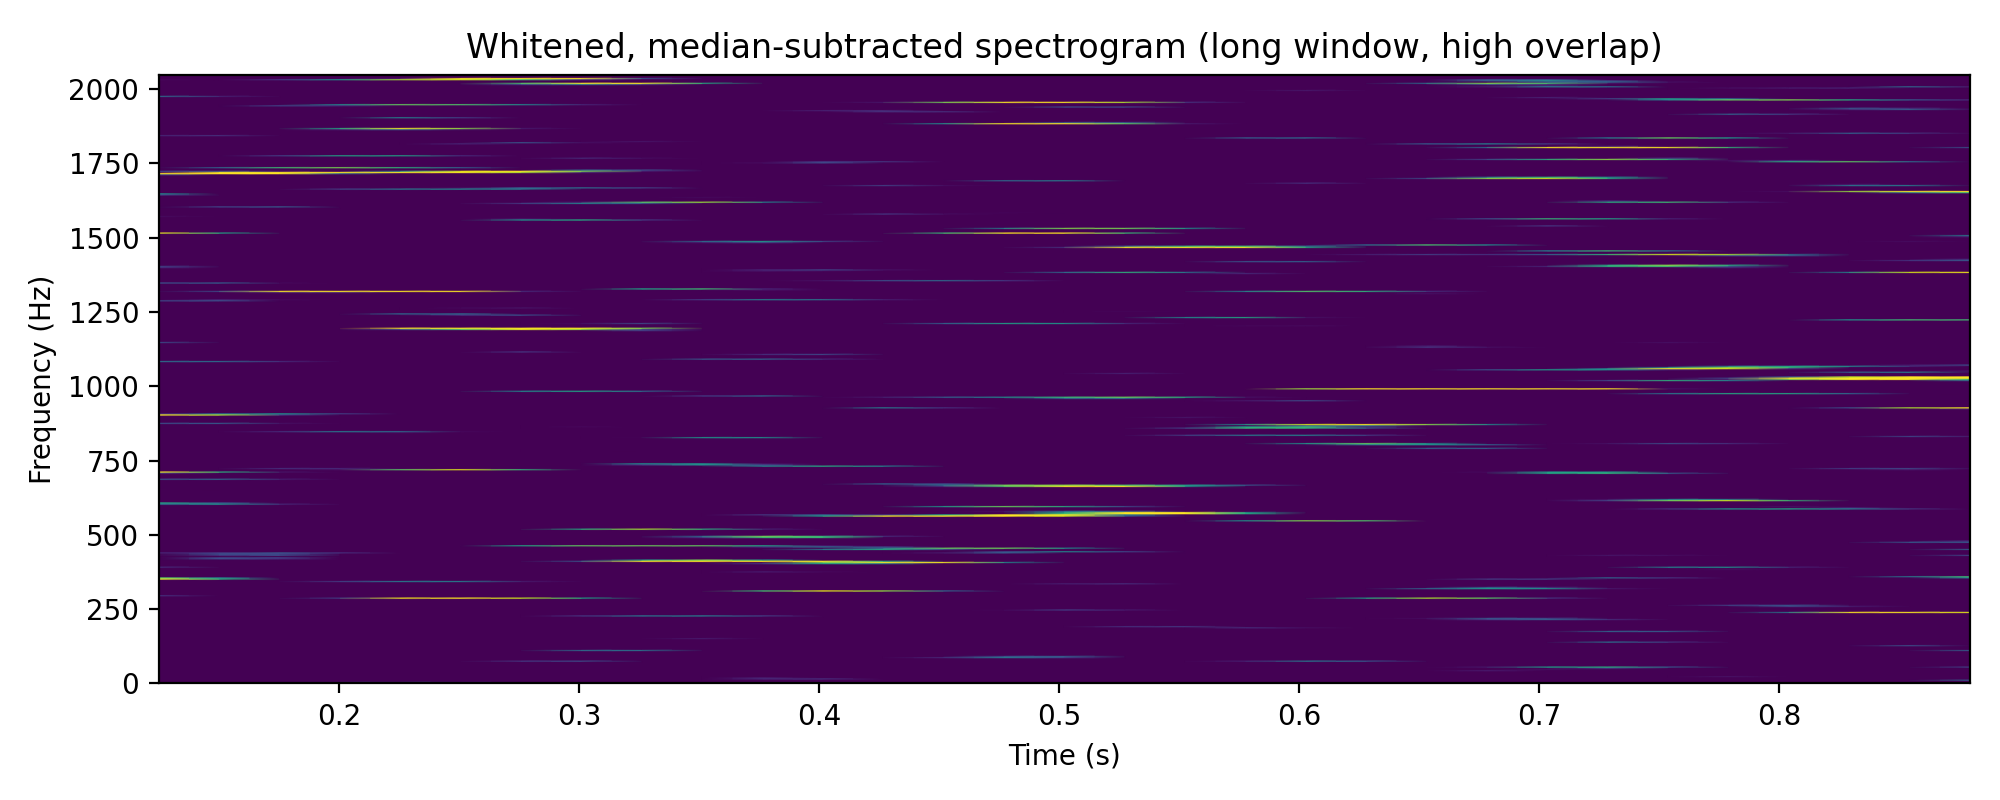
\includegraphics[width=0.95\linewidth]{fig4_spectrogram.png}
\caption{Whitened, median-subtracted spectrogram computed with a long Hann window and 90\% overlap. The color limits are clipped to the 95th--99.5th percentiles to reduce variance and enhance contrast.}
\label{fig:spec}
\end{figure}

\section{From Toy to Observatory: What We Simplified}
Our toy omits engineering details: robust PSD tracking, whitening of very long records, banks of many templates, coherence across detectors, and false-alarm estimation via time shifts. The core ideas, however, remain those expressed by Eqs.~\eqref{eq:h0}--\eqref{eq:stft}.

\appendix
\section*{Appendix A: Parameters}
\noindent The experiment parameters used in the figures are collected in Table~\ref{tab:params}.
\begin{table}[h!]
\centering
\caption{Parameters of the toy experiment.}
\label{tab:params}
\begin{tabular}{ll}
\toprule
Parameter & Value \\
\midrule
Sampling rate & 4096 Hz \\
Duration & 1.00 s \\
Chirp start frequency & 30.0 Hz \\
Chirp end frequency & 300.0 Hz \\
Signal amplitude & 0.50 \\
Noise std. dev. & 0.50 \\
Estimated arrival time & 0.1643 s \\
Approx. SNR (toy) & 3.38 \\
Residual μ, σ & 0.008, 0.498 \\
\bottomrule
\end{tabular}

\end{table}

\section*{Appendix B: Reproducibility Notes}
Upload this \LaTeX{} file with the images and \texttt{parameters.tex} to Overleaf. The Python code that generated the figures is available separately.

\end{document}
